%!TeX root=../tese.tex
%("dica" para o editor de texto: este arquivo é parte de um documento maior)
% para saber mais: https://tex.stackexchange.com/q/78101

%% ------------------------------------------------------------------------- %%

% "\chapter" cria um capítulo com número e o coloca no sumário; "\chapter*"
% cria um capítulo sem número e não o coloca no sumário. A introdução não
% deve ser numerada, mas deve aparecer no sumário. Por conta disso, este
% modelo define o comando "\chapter**".
\chapter{Introdução}
\label{cap:introducao}

\enlargethispage{.5\baselineskip}

Grafos são estruturas de dados que nos permitem modelar vários problemas existentes da vida real, sejam eles estáticos ou dinâmicos. Em problemas estáticos, o grafo não sofre alterações com o passar do tempo. Podemos citar, como exemplo, o planejamento de rotas de entrega, análise de moléculas químicas e de dependências em software utilizando ordenação topológica. Entretanto, ainda existem muitas situações em que ocorre dinamicidade, como nas interações de usuários em redes sociais, monitoramento de epidemias (contatos e isolamentos) e sistemas de navegação \textit{GPS}, onde há necessidade de recalcular rotas dependendo das condições como congestionamentos e acidentes. Para modelar tais problemas, usamos grafos dinâmicos para modelá-los.

Dessa forma, são considerados problemas em grafos completamente dinâmicos aqueles em que o grafo sofre, com o tempo, alterações como inserções e remoções 
de arestas. Caso o algoritmo permita apenas inserção ou apenas remoção, tais 
problemas são chamados de parcialmente dinâmicos, conforme Holm, de Lichtenberg e Thorup \cite{jacob_holm}. Note que as operações de 
atualização e consulta são apresentadas de forma online, sem conhecimento algum das operações futuras.

Aqui serão tratados problemas em que o grafo dinâmico possui um conjunto fixo de vértices \textit{V}, e estabelecemos $n = |\textit{V}\ |$. Além disso, pode-se definir $m$ como o número de arestas existentes. Na maior parte das vezes, a complexidade de tempo das operações será amortizada, o que implica que elas são calculadas como a média sobre todas as operações realizadas. 


Um grafo dinâmico de ordem n é uma sequência de grafos ($G_0$, $G_1$, $\cdots$, $G_T$), onde $G_0$ é o grafo inicial com \textit{n} vértices e cada $G_t$ para $1 \leq t \leq T$ é obtido a partir de $G_{t-1}$ pela adição ou remoção de uma aresta. Assim, podemos escrever $E(G_{t}) := E(G_{t - 1}) \setminus \{uv\}$, para alguma aresta $uv \in E(G_{t-1})$. Chamamos de \textbf{alterações}, \textbf{modificações} ou \textbf{atualizações} quando ocorre alguma operação de adição e/ou remoção de arestas no grafo dinâmico.

Um problema em grafos dinâmicos consiste em verificar se o grafo atual \textit{G} satisfaz alguma propriedade, e cada operação que realiza essa verificação é denominada \textbf{consulta}. A solução do problema depende da criação de um algoritmo que utiliza uma estrutura de dados capaz de realizar estas consultas e as alterações de forma eficiente. 

Um problema clássico em grafos é o problema da árvore geradora de custo mínimo (MST, de \textit{Minimum Spanning Tree}). Para defini-lo, iremos introduzir alguns conceitos em grafos. Seja um grafo conexo não dirigido $G = (V, E)$. onde $V$ é o conjunto de vértices e $E$ o conjunto de arestas. Um grafo não-dirigido significa que para qualquer aresta $uv \in E$, podemos ir de $u$ a $v$ e vice-versa, ou seja, a aresta não possui direção. Para cada aresta $uv \in E$, temos um peso $w(uv)$ associado. Então queremos encontrar um subconjunto acíclico $T \subseteq E$ que conecte todos os vértices e que o peso total 

$$
w(T) = \sum_{e \,\in\, E(T)} w(e)
$$
seja minimizado. Como $T$ é acíclico e conecta todos os vértices, então temos uma árvore, o qual denominaremos \textbf{árvore geradora de custo mínimo}, visto que é uma árvore que ''gera'' o grafo e estamos interessados em conectar todos os vértices de modo que o peso das arestas utilizadas tenham a menor soma possível. O problema de determinar a árvore $T$ se chama problema da árvore geradora de custo mínimo. A Figura 1.1 mostra um exemplo de grafo conexo e uma árvore geradora mínima de peso 17.

\begin{figure}
    \centering
    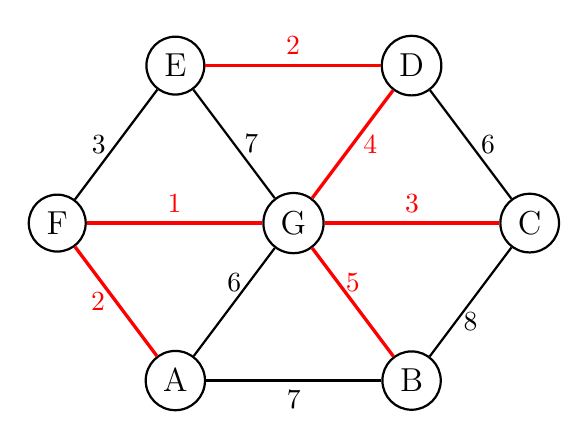
\begin{tikzpicture}
        [node/.style={circle,draw,minimum size=2em, thick, font=\large},
        edge/.style={thick},
        mst/.style={very thick, red}]
        
        % Vertices in a circular arrangement
        \node[node] (A) at (0,0) {A};
        \node[node] (B) at (3,0) {B};
        \node[node] (C) at (4.5,2) {C};
        \node[node] (D) at (3,4) {D};
        \node[node] (E) at (0,4) {E};
        \node[node] (F) at (-1.5,2) {F};
        \node[node] (G) at (1.5,2) {G};
        
        % Non-MST edges (normal black edges)
        \draw[edge] (A) -- (B) node[midway, below] {7};
        \draw[edge] (B) -- (C) node[midway, below] {8};
        \draw[edge] (C) -- (D) node[midway, right] {6};
        \draw[edge] (A) -- (G) node[midway, above] {6};
        \draw[edge] (E) -- (G) node[midway, right] {7};
        \draw[edge] (F) -- (E) node[midway, left] {3};
        
        % MST edges (highlighted in red)
        \draw[mst] (A) -- (F) node[midway, left] {2};
        \draw[mst] (G) -- (D) node[midway, right] {4};
        \draw[mst] (F) -- (G) node[midway, above] {1};
        \draw[mst] (G) -- (C) node[midway, above] {3};
        \draw[mst] (E) -- (D) node[midway, above] {2};
        \draw[mst] (B) -- (G) node[midway, above] {5};
        
    \end{tikzpicture}
    \caption{Um grafo não-direcionado com 7 vértices. As arestas em vermelho formam uma árvore geradora mínima (MST) de peso total 17.}
    \label{fig:mst_example}
\end{figure}

Existem diversas famílias de grafos, de modo que cada uma é adequada para resolver um tipo de problema particular. Iremos tratar inicialmente do \textbf{problema de conexidade em grafos dinâmicos}, que consiste em manter um grafo dinâmico que sofre uma sequência de inserções e remoções de arestas. Entre essas modificações, realizamos consultas para verificar se dois vértices \textit{u} e \textit{v} estão conectados por algum caminho. Para este problema, iremos usar as \textbf{florestas} (coleção de árvores) como base para a construção do algoritmo.

Inicialmente, utilizaremos o \textbf{problema de conexidade em florestas dinâmicas} como base para construir o algoritmo do \textbf{problema de conexidade em grafos dinâmicos}, e, a partir este, construir o \textbf{algoritmo decremental para árvores geradoras de custo mínimo}. Tais problemas possuem soluções propostas por \textit{Holm, de Lichtenberg e Thorup} \cite{jacob_holm}, nas quais a nossa implementação será baseada, e usaremos \textit{C++} como linguagem do código, onde disponibilizamos no repositório do \textit{GitHub} \cite{chung2025}.